\begin{figure}[htbp]
\centering
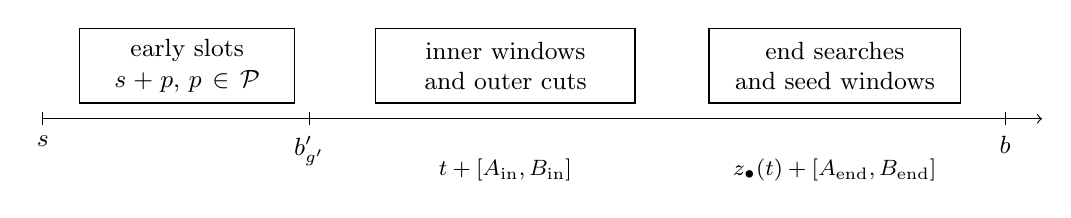
\begin{tikzpicture}[x=.94cm,y=1cm,font=\small]
 \draw[->] (0,0)--(13.5,0);
 \draw (0,-.08)--(0,.08) node[below=5pt] {$s$};
 \draw (13,-.08)--(13,.08) node[below=5pt] {$b$};
 \draw (.5,.2) rectangle (3.4,1.15);
 \node[text width=2.5cm,align=center] at (1.95,.675)
   {early slots\\$s+p$, $p\in\mathcal P$};
 \draw (4.5,.2) rectangle (8,1.15);
 \node[text width=3cm,align=center] at (6.25,.675)
   {inner windows\\and outer cuts};
 \draw (9,.2) rectangle (12.4,1.15);
 \node[text width=2.9cm,align=center] at (10.7,.675)
   {end searches\\and seed windows};
 \draw (3.6,-.08)--(3.6,.08) node[below=5pt] {$b'_{g'}$};
 \node[font=\footnotesize,align=center] at (6.25,-.65)
   {$t+[A_{\rm in},B_{\rm in}]$};
 \node[font=\footnotesize,align=center] at (10.7,-.65)
   {$z_\bullet(t)+[A_{\rm end},B_{\rm end}]$};
\end{tikzpicture}
\caption{The order of bounded data in a complete episode, schematically
and not to scale.  Both window intervals include every prescribed shifted
hypothesis.  The end anchor may be a bounded marker return or a later
first mismatch; in either case the fixed tail puts $b$ beyond all bounded
end data.}\label{schedule:schematic}
\end{figure}
